%-*- coding: utf-8 -*-
\section{提案手法の概要}
小松らの手法を基に,早上がりについても考慮するようにプレイアウトの報酬値を改良する.手牌とランダムに仮定した残り巡目数分の牌から,報酬が最大となる組み合わせを求めることは変わらない.また,求めた組み合わせに含まれない手牌の牌に,報酬を与える部分も同様である.小松らの手法では報酬を上がり点をしていたところを,次節で説明する報酬値とする.
\section{報酬値の計算}
求めた組み合わせの上がり点を$P$としたとき,小松らの手法の報酬$R_{komatu}$は以下のようになる.
\begin{equation*}
R_{komatu}=P
\end{equation*}
提案手法では,求めた組み合わせで使われている手牌の牌の使用枚数$U$を報酬に用いる.元の手牌の牌の集合を$T$,求めた組み合わせの牌の集合を$T'$としたとき,$U=|T \cap T'|$とする.提案手法は報酬$R$を以下のようにする.
\begin{equation}
R=\alpha*(P/48000)+(1-\alpha)*(U/13)
\label{reward}
\end{equation}
$\alpha$はバランスパラメータである.式~\ref{reward}の第1項は,上がり点の最大値である48000で正規化している~\cite{point}.第2項は,求める組み合わせで使われる手牌の牌の使用最大枚数である13で正規化している.報酬に$P$を用いることで上がり点を高くするように捨てる牌を選び,$U$を用いることで早く上がるように捨てる牌を選ぶようになる.$P$については小松らの手法から高い上がり点を目指すようになることは確かである.$U$についてだが,この値が大きいとき,求めた組み合わせと手牌の変化枚数が少ないことになる.早上がりを目指すならば,変化枚数の少ない組み合わせを作るように打つのが良い.組み合わせに含まれていない手牌の牌に,$U$を報酬として与えることで,その牌が選ばれやすくなり,早上がりを目指すようになる.この報酬を使ったプレイアウトについて例を使って説明する.図~\ref{tehaifuture}の手牌と仮定した牌でできる組み合わせの例を図~\ref{excombination}にいくつか示す.一番上の例が報酬として最大だった場合,組み合わせに含まれない手牌の牌の七萬に報酬として$\alpha*(1500/48000)+(1-\alpha)*(13/13)$を与える.また,提案手法の疑似コードをAlgorithm~\ref{proposal}に示す.この手法により,$\alpha$の値を変えることで,高得点を優先するか早上がりを優先するか打ち方を変えることができる.

\begin{figure}[t]
	\begin{center}
		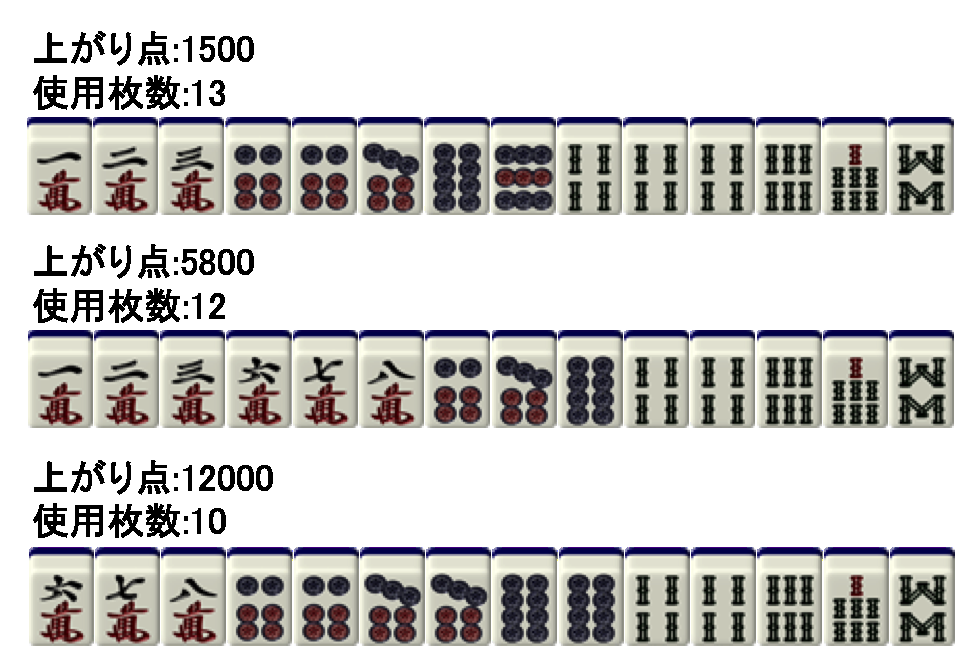
\includegraphics{fig/excombination.eps}
	\end{center}
	\caption{図~\ref{tehaifuture}の牌でできる組み合わせの例}
	\label{excombination}
\end{figure}

\begin{algorithm}[t]
\caption{提案手法}
\label{proposal}
	\KwIn{手牌$T$}
	価値を格納する要素数14の配列$V$の各要素を0にする\;
	\For{$i=1$ \KwTo $N$}{
		残り巡目数分の牌をランダムに仮定する\;
		$\alpha*(P/48000)+(1-\alpha)*(U/13)$が最大となる組み合わせを求める\;
		\For{$j=1$ \KwTo $14$}{
			\If{$j$番目の牌が組み合わせに含まれない}{
				$V_j \leftarrow V_j + R$\;
			}
		}
	}
	$s \leftarrow \argmax_{1 \le j \le 14} V_j$\;
	\Return $T_s$\;
\end{algorithm}
